\chapter{Ergebnisse}
\label{chap:ergebnisse} Dieses Kapitel präsentiert alle Ergebnisse, die in
dieser Arbeit erzielt wurde. Dabei spielen nicht nur die erfolgreichen Ziele eine
Rolle, sondern auch die Misserfolge. Zunächst wird die entwickelte Erweiterung in
seiner finalen Form beschrieben, gefolgt von einer Darstellung der zentralen
Funktionen. Anschließend wird auf die Konzeptionen und Umsetzungen der verschiedenen
Teile eingegangen. Abschließend soll die Performance und die verschiedenen
Anwendungsszenarien genauer analysiert werden. Daraus ergeben sich auch Limitierungen
für die Software. Mit diesen erstellten Analysen kann unter Berücksichtigung
eine Aussage bezogen auf die Forschungsfrage gestellt werden.
% ---------------------------------------------------------------------------------------

\section{Tooth Analyser}
\label{sec:tooth_analyser} Im Rahmen dieser vorliegenden Arbeit ist eine 3D
Slicer Extension entstanden, die den Namen Tooth Analyser trägt und für die Forschung
im Dentalbereich eingesetzt wird. In erster Linie können mit diesem Plugin Micro
CT Aufnahmen anatomisch segmentiert werden. Das Modul schmiegt sich wie alle anderen
Module gut in die Kernanwendung ein und ist auch für die aktuelle stabile Version
von Slicer (v5.8.0) verfügbar. Neben der eigentlichen Implementierung ist auch
ein Logo für das Plugin entstanden, das es nach außen repräsentiert. Die
Abbildung \ref{fig:logo_tooth_analyser} zeigt dies.

\begin{figure}[h]
	\centering
	
\includegraphics[width=0.9\textwidth]{img/SlicerToothAnalyser.png}
	\caption{Logo der 3D Slicer Erweiterung "Tooth Analyser", welche im Rahmen dieser
	Arbeit entwickelt wurde. Logodesign: Dr. Elias Walter}
	\label{fig:logo_tooth_analyser}
\end{figure}

Des Emblem des Tooth Analyser bildet einen Zahn ab, dessen Hauptsegmenten (Schmelz,
Dentin, Pulpa) mit den unterschiedlichen Farben (grün, gelb, orange)
visualisiert werden. Dies verdeutlicht die Analogie zur anatomischen Segmentierung
und lässt gleich vermuten, dass sich dieses Modul mit einer Segmentierung
beschäftigt. Der Untertitel deutet konkret auf Micro \ac{CT} Aufnahmen geht. Wurde
der Tooth Analyser installiert, so ist er über den Menüpunkt Module in Slicer
auswählbar. Hier wird er in dem Unterpunkt \textit{Segmentierung} eingruppiert, was
ein weiteres Indiz auf die grobe Funktionalität liefert. Wird also der Tooth
Analyser gestartet so erhält man die Ansicht der Kernanwendung mit der
Entsprechenden \ac{UI}. Die Abbildung \ref{fig:tooth_analyser_start_up} soll
genau diese Ansicht verdeutlichen

\begin{figure}[h]
	\centering
	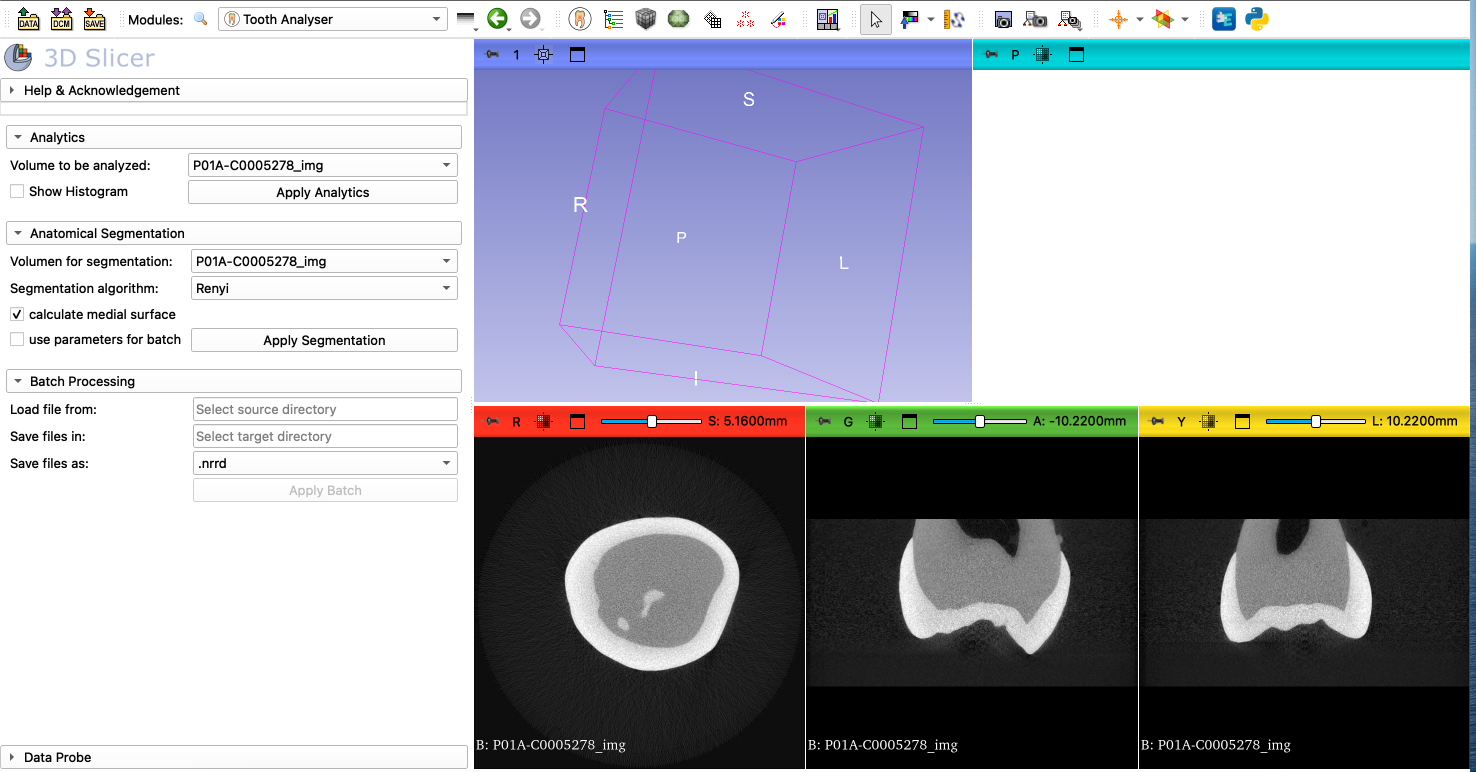
\includegraphics[scale=0.2, width=\textwidth]{img/toothAnalyserStarUp.png}
	\caption{Startansicht der Erweiterung Tooth Analyser nach dem ersten Aufruf}
	\label{fig:tooth_analyser_start_up}
\end{figure}

Die Ansicht zeigt die Kernanwendung (rechts die verschiedenen Fenster) und die
\ac{UI} des jeweiligen Moduls. Die Kernanwendung kann auch als Szene beschrieben
werden und übernimmt alle generischen Handhabungen der Bilder. Neben den Szenen ist
auch immer eine Sidebar zu sehen, welche die \ac{UI} des jeweiligen Moduls abbildet.
Im Falle der Abbildung \ref{fig:tooth_analyser_start_up} ist es die \ac{UI} des Tooth
Analyser. Das manuelle Laden eines Bildes in die Szene ist Teil der Slicer
Kernanwendung und nicht teil der Modullogik. Das bereits geladene Bild ist demnach
unabhängig von der Slicer Erweiterung entstanden. Betrachtet man die
Benutzerschnittstelle genauer, so fällt sofort auf, dass diese in vier Bereiche
unterteilt ist. Diese Aufteilung in Bereiche ist ein Ergebnis der Literaturrecherche
und eine gute Konvention in der Welt von 3D Slicer. Der Bereich \textit{Help and
Acknowledgement} stellt Hilfen und Informationen über das Modul bereit. Über
diesen Abschnitt ist auch die offizielle Dokumentation über dieses Modul
erreichbar. Zu Beachten ist, dass dieser Bereich nicht eigens für den Tooth
Analyser entwickelt wurde. Es handelt sich hier um eine Funktionalität, die
automatisch allen \ac{SEM} zur Verfügung steht. Bei den übrigen Abschnitten
handelt es sich im Features die spezifische für den Tooth Analyser entwickelt
wurden. Bevor genauer auf die Funktionalitäten des Tooth Analyser eingegangen wird,
sei zunächst auf die Abbildung \ref{fig:tooth_analyser_full_view} verwiesen, welche
die Ergebnisansicht zeigt.

\begin{figure}[h]
	\centering
	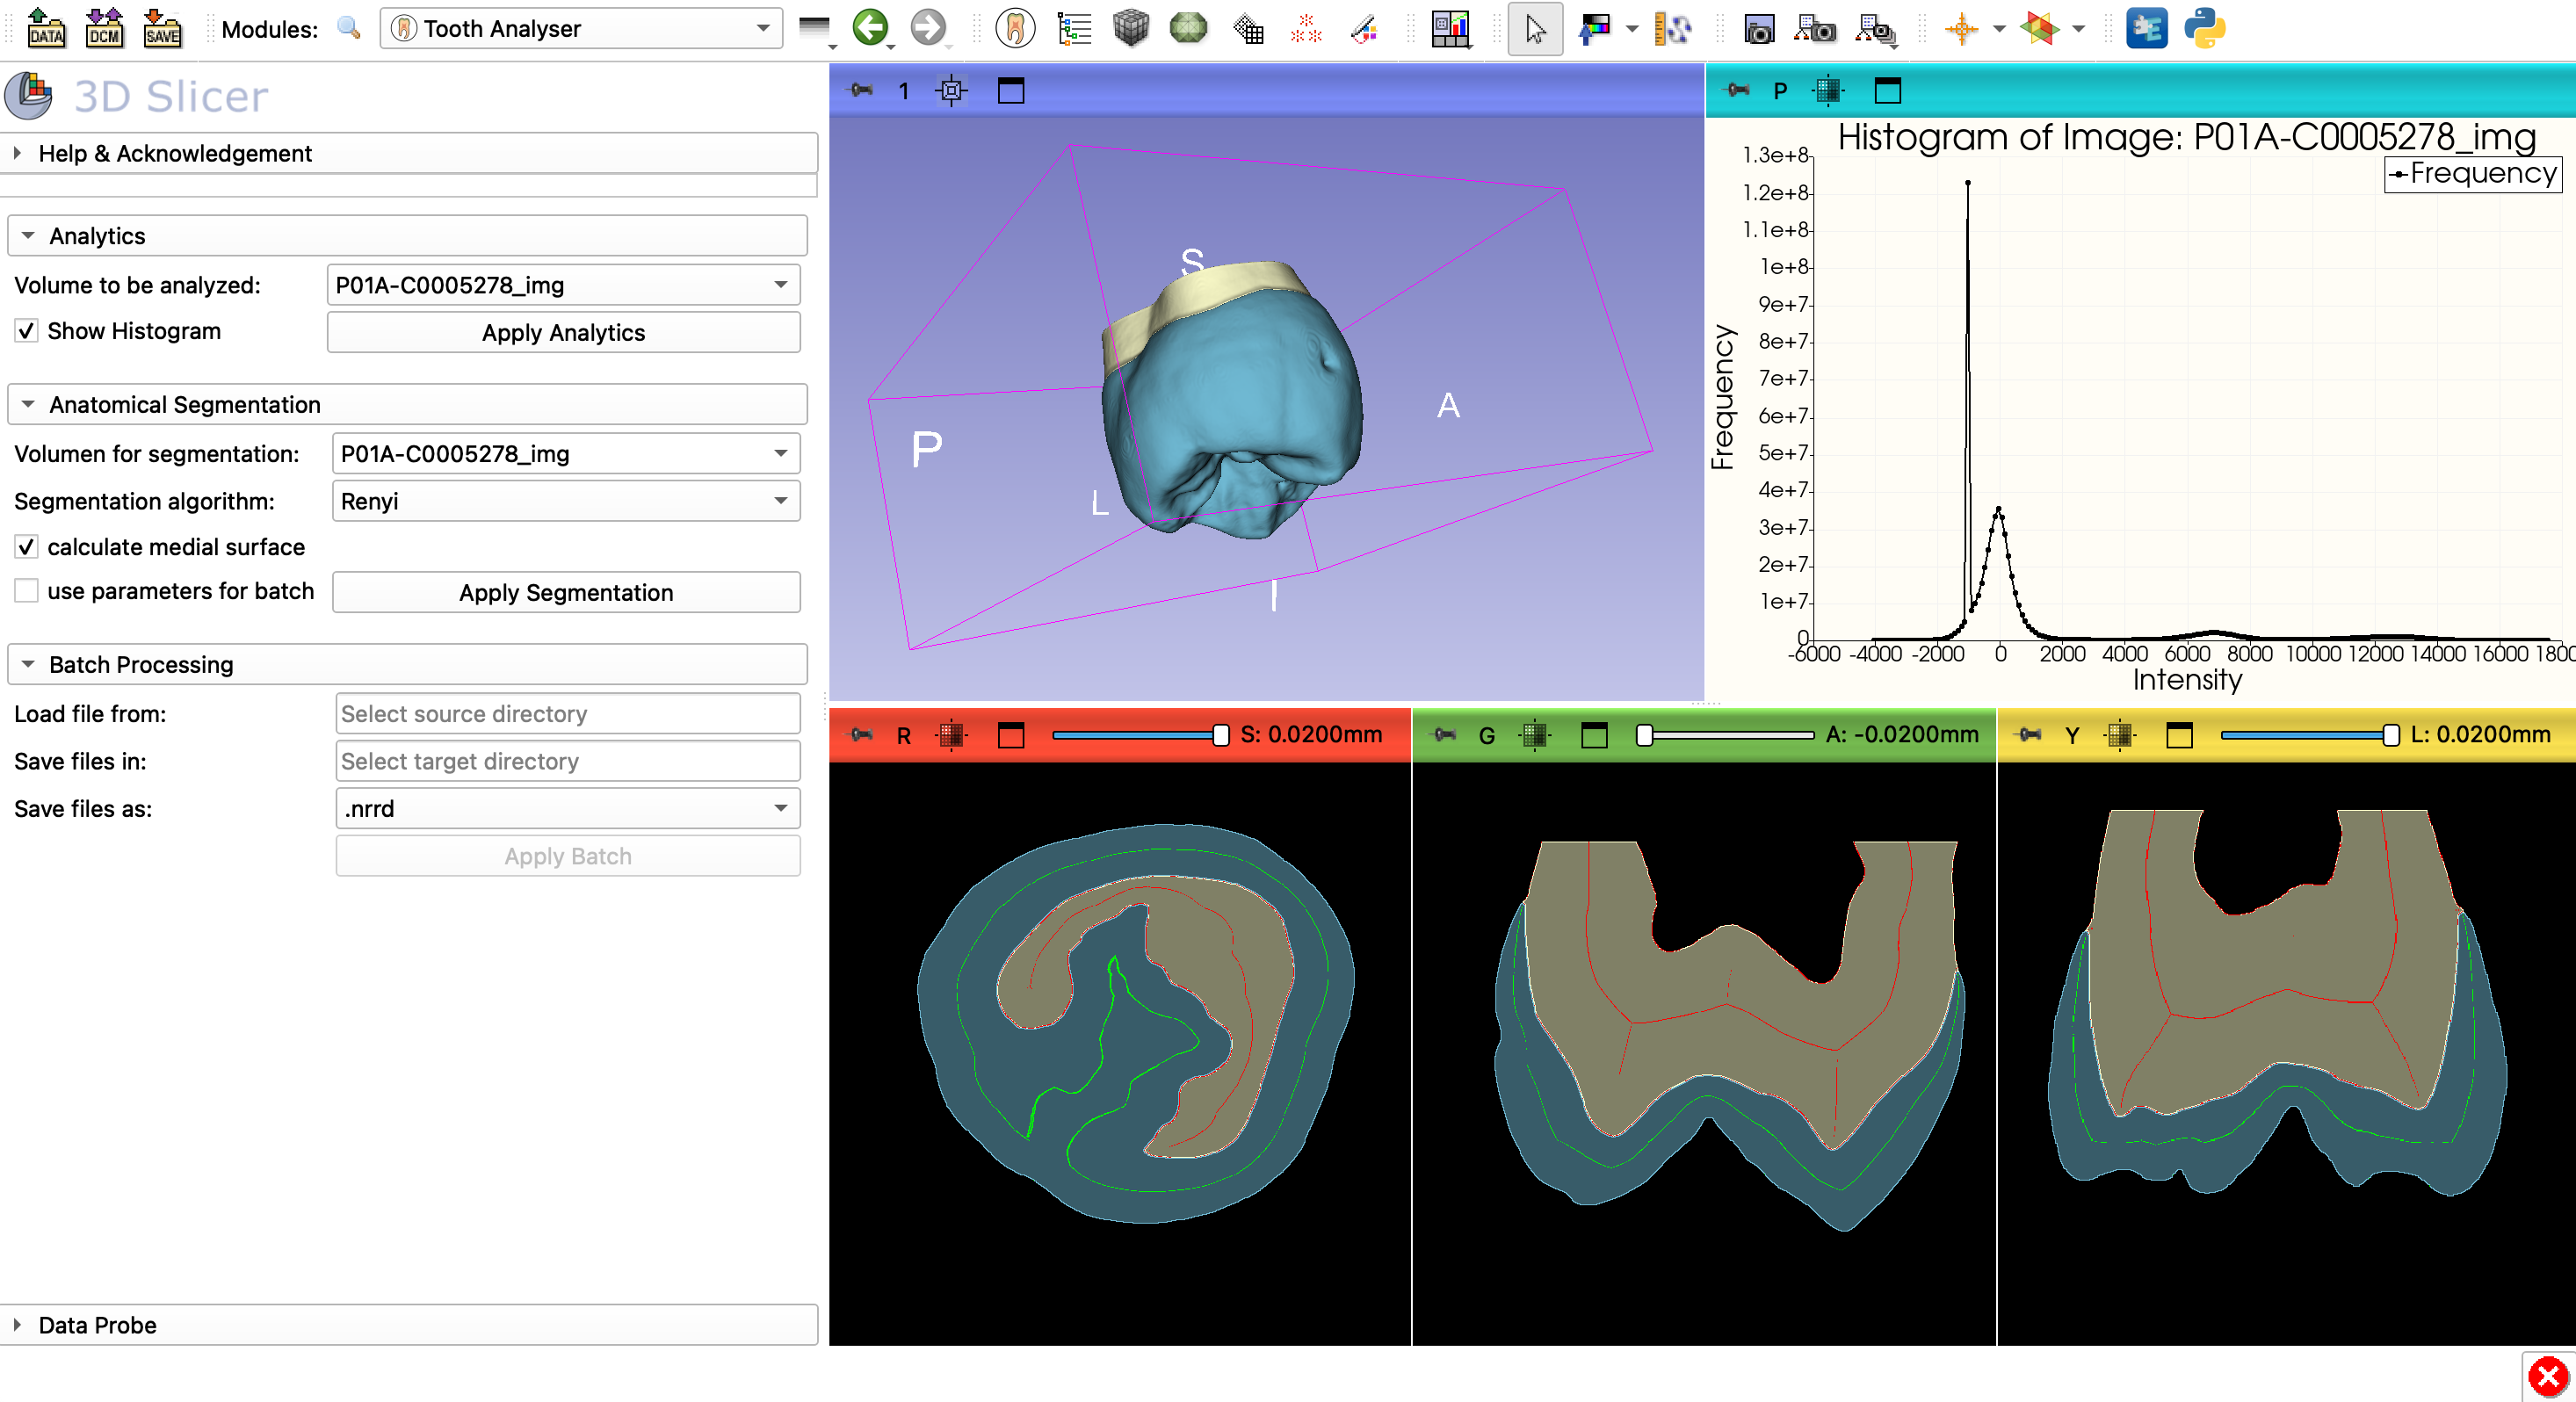
\includegraphics[scale=0.2, width=\textwidth]{img/toothAnalyserFullView.png}
	\caption{Ergebnisansicht der Erweiterung Tooth Analyser, nachdem die Analysen und
	die anatomische Segmentierung erstellt wurden.}
	\label{fig:tooth_analyser_full_view}
\end{figure}

Der Analysebereich des Tooth Analyser ermöglicht es das Histogramm eines
gegebenen Bildes zu erstellen. Dies ist besonders interessant, wenn ein
Algorithmus für die anatomische Segmentierung ausgewählt werden muss. Diese Algorithmen
sind Schwellwertverfahren, die auf das Histogramm eines Bildes basieren, um es zu
segmentieren. Das erstellte Histogramm ist rechts oben in der Abbildung
\ref{fig:tooth_analyser_full_view} zu erkennen. Es wird in einem Plot-Node dargestellt
und kann über diesen auch verändert werden. Hierzu ist die Pinnnadel im Fenster
des Plot-Node zu wählen. Durch die Speicherfunktion der Kernanwendung kann der Plot
auch problemlos gespeichert werden. Bevor die Analysen erstellt werden können, müssen
Parametereinstellungen gewählt werden. Hierbei ist der wichtigste Parameter der,
indem das konkrete Bild ausgewählt wird. Bei diesem Parameter handelt es sich um
ein Dropdown, indem nur Bilder mit dem Typ \texttt{vtkMRMLScalarVolumeNode}
ausgewählt werden können. Dies trägt zur Stabilität und Ausfallsicherheit des Systems
bei und sorgt dafür, dass nicht jedes beliebige Bild geladen werden kann. Ist keine
\ac{CT} Aufnahme ausgewählt, so bleibt der Button zum Starten der Analysen deaktiviert.
Wird ein Bild in die Szene geladen, während der Parameter für das zu analysierende
Bild leer ist, wählt der Tooth Analyser automatisch das Bild aus, dass als Erstes
in die Szene geladen wurde. So spart der Benutzer einige Klicks. Durch die Checkbox
\textit{Show Histogram} wird der Erweiterung signalisiert das beim Starten der
Analysen ein Histogramm des übergebenen Bildes erstellt werden soll.

Die Hauptfunktionalität des Tooth Analyser ist die anatomische Segmentierung
welche in Kapitel \ref{sec:verwwandte_arbeit} detailliert erläutert wurde. Die konkreten
Ergebnisse dieser Segmentierung sind in der Abbildung \ref{fig:tooth_analyser_full_view}
in den Fenstern (blau, rot, grün, gelb) zu sehen. Neben der eigentlichen Segmentierung
sind auch hier die medialen Flächen für die Segmente Dentin (rot) und Schmelz (grün)
gut sichtbar. Hinzu kommt ein \ac{3D} Modell, das auf Basis der erstellten
Segmentierung generiert wurde und nur der Visualisierung dient. Ein Abspeichern dieses
3D Modells als Netz ist nicht möglich. Um überhaupt eine anatomische
Segmentierung eines Zahnes erstellen zu können, sieht der Algorithmus zunächst drei
Parameter vor, die eingestellt werden müssen. Um die Komplexität gering zu halten,
wurde bewusst auf viele Parameter verzichtet. Ähnlich wie bei den Analysen ist auch
hier die Wahl des zu segmentierenden Volumens der entscheidende Parameter.
Dessen Bedeutung gleicht der Analysen, insbesondere in Bezug auf das Verhalten.
Damit schnell ein Ergebnis generiert werden kann, wurde für die übrigen zwei Parameter
eine Vorauswahl definiert, die zum vollen Ergebnisumfang des Tools führt. So ergibt
sich die Situation, das nach dem Laden eines \ac{CT}s in die Szene nur auf den
Button für das Ausführen gedrückt werden muss, damit eine anatomische Segmentierung
erstellt wird. Dies nimmt dem Benutzer viel Arbeit ab und sorgt für eine gut \ac{UX}.
Sind jedoch Einstellungen in den Parametern gewünscht, so können diese natürlich
getätigt werden. Über den Parameter \textit{Segmentation algorithm} kann das entsprechenden
Schwellwertverfahren gewählt werden, mit dem der Zahn segmentiert werden soll. Dies
mag nur geringfügig eine Änderung auf die Ergebnismenge ausmachen, kann aber
dennoch wichtig sein. Die Checkbox \textit{calculate medial surface} ermöglicht
eine optionale Erstellung der medialen Flächen. Wird diese Funktion ohnehin nicht
gebraucht, so kann diese hier ausgelassen werden und damit Laufzeit eingespart
werden.

Die letzte Funktionalität, die geboten wird, stellt kein neues Verfahren dar, sondern
nur eine andere Art der Ausführung. Die Rede ist hier von einem Batch Modus, der
nicht nur ein Bild segmentiert, sondern das Verfahren der anatomischen
Segmentierung auf eine ganze Reihe an Bildern anwendet. Um diesen Modus aktiv zu
schalten, muss neben den Parametern im Abschnitt \textit{batch} auch die Checkbox
\textit{use parameters for batch} aktiviert werden. Der Tooth Analyser überträgt
dann die aktuellen Parametereinstellungen der anatomischen Segmentierung an den Batch
Modus. Um dann den Batch Modus ausführen zu können, müssen noch zwei Pfade angegeben
werden, die jeweils zu einem Ordner führen. Diese beiden Pfade teilen sich auf in
\textit{source} und \textit{target} und geben an, wo die Daten liegen, die segmentiert
werden soll und wo die segmentierten Daten auf der Festplatte gespeichert werden.
Abschließend ist hier noch zu wählen in welchem Format die erstellten Daten
abgespeichert werden sollen. Bei diesem Feature ist zu beachten, dass nach
Erfolgreichem ausführen keine Daten in der Slicer Szene geladen werden. Der Prozess
läuft im Hintergrund und ist bis auf die Parametereinstellung über die UI komplett
getrennt von Slicer. Nach Ende des Batch Modus wird in dem angegebenen
Zielordner ein Unterordner erstellt, der alle Dateien der segmentierten Bilder enthält.
Hierfür sieht der Tooth Analyser weitere Unterordner für jedes segmentierte Bild
vor. Ein automatisches Laden aller segmentierten Bilder nach dem Batch Prozess ist
nicht implementiert, sodass der erstellte Ordner mit allen Segmentierungsdaten
manuell über den Import geladen werden muss.

Da neben der reinen Erstellung noch weitere Anforderungen an die Erweiterung
gegeben waren, beschäftigt sich die nächsten Kapitel tiefer mit den softwaretechnischen
Aspekten des Tooth Analyser. Hierzu sollen auch die einzelnen Teilaufgaben, die zu
Beginn definiert wurden, wieder aufgegriffen werden.
% ---------------------------------------------------------------------------------------

\section{Konzeptionen}
\label{sec:konzeptionen} Die ausgearbeiteten Konzeptionen bilden überwiegend die
Ergebnisse der in \ref{sec_zerlegung_in_teilprobleme} beschriebenen Teilaufgaben.
Konkret soll das bedeuten, dass hier konzeptionell gezeigt wird, wie die softwaretechnischen
Aspekte aus den Anforderungen umgesetzt wurden. Hierzu soll zunächst das Design-Klassendiagramm
betrachtet werden, das sich aus dem Domänenmodell in Abbildung \ref{fig:3d_slicer_domäne}
ableiten lässt.

KLASSENDIAGRAMM - BILD

Wie das Diagramm zeigt, ist die Anwendung über die Klasse \texttt{ToothAnalyserWidget}
in das Kernsystem eingebunden. Sie hält auf der einen Seite alle Parameter der verschiedenen
Funktionen und auf der anderen Seite die dazugehörigen Logiken. Des Weiteren
bildet diese Klasse die gesamt UI des Tooth Analyser ab, was unter anderem das Laden
der \ac{UI} mit einschließt. Die UI des Tooth Analyser wurde mit der Software QT-Designer
erstellt und dann mittels einer Methode in die Anwendung geladen. Nachfolgend
sei der Designentwurf für die \ac{UI} gezeigt.

\begin{figure}[h]
	\centering
	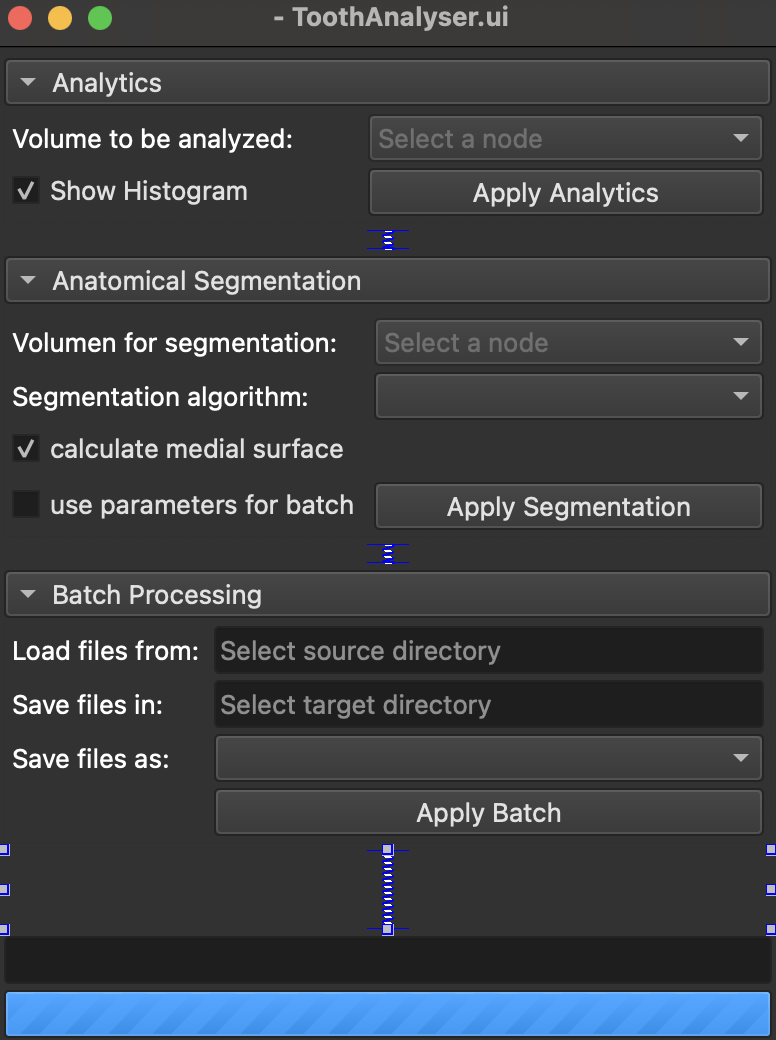
\includegraphics[width=0.4\textwidth]{img/toothAnalyserQT.png}
	\caption{Bearbeitungsansicht der \ac{UI} des Tooth Analyser im QT-Designer}
	\label{fig:tooth_analyser_qt}
\end{figure}

Wie auch schon im Kapitel \ref{sec:tooth_analyser} beschrieben teilt sich die
\ac{UI} auch hier sichtbar in unterschiedliche Teile auf. Vergleicht man nun
Abbildung ... mit dem Klassendiagramm aus Abbildung ... so fällt auf, das Für jeden
Funktionsbereich eine eigene Parameterklasse erstellt wurde, die dann wiederum
in der Klasse ParameterNode zusammengefasst werden. Dies stellt eine gute Erweiterbarkeit
der \ac{UI} um zusätzliche Parameter sicher. Es wurde an dieser Stelle bewusst keine
Generalisierung verwendet, da Slicer genau diesen konzeptionierten Mechanismus
vorsieht. Auf der anderen Seite der Struktur finden sich die Logikklassen. Die
verschiedenen Logiken die aktuell und zukünftig den Tooth Analyser ausstatten, verwenden
alle dieselbe Schnittstelle, die über die Klasse \texttt{ToothAnalyserLogic} bereitgestellt
wird. Soll also in Zukunft weitere Funktionen hinzukommen, so kann hier einfach eine
weitere Klasse an die Schnittstelle angehängt werden. So entsteht etwas was man
in der Fachliteratur als \textit{Strategy Pattern} bezeichnet \citep[vgl.][S. ...]{siebler2014}.
Der Bentuzer der Software wählt also über die verschiedenen Buttons aus, welche
Strategie er gerade nutzen will. Der Tooth Analyser sorgt dann dafür, dass auch
die richtige Funktion geladen wird. Das Feature für den Batch Modus funktioniert
nach einem anderen Schema. Da dieser Modus auch für alle zukünftigen Funktionen
gelten soll, wird dieser nicht als eigene Strategie, sondern direkt in der
Schnittstelle bereitgestellt. So ist sichergestellt, dass eine Implementierung
erfolgen muss, sie jedoch für alle Strategien unterschiedlich sein kann. Um noch
etwas genauer zu zeigen, welche Schritte notwendig sind um den Tooth Analyser mit
weiteren Funktionen auszustatten sei auf Abbildung ... verwiesen. Hier wird
deutlich, welche Klassen und Methoden erstellt werden müssen

KLASSENDIAGRAMM NEUE FUNKTION - BILD

Wie bereits zu erkennen ist, signalisieren die roten Elemente die Punkte, an denen
die Funktionalität erweitert werden kann. Die gestrichelte, rote Linie verdeutlicht
nur den Zusammenhang dieser Komponenten und hat keine Auswirkung auf die Konzeption.
Um einen noch genaueren Einblick in die Strukturen zu geben, geht das nachfolgende
Kapitel noch einen Schritt weiter und geht auf konkrete Implementierungsdetails ein.

% ---------------------------------------------------------------------------------------

\section{Technische Umsetzung}
\label{sec:technische_umsetzung} Zu Beginn sei gesagt, dass dieses Kapitel nicht
alle Funktionen detailliert beschreibt, sondern sich auf die wichtigsten
Funktionen und Methode des Tooth Analyser beschränkt. Eine Grobe Übersicht über die
Wichtigsten Klassen soll zu Begin die Tabelle \ref{tab:methoden_klassen} liefern.
Die Reihenfolge gibt eine grobe Orientierung bezüglich der Wichtigkeit.

\begin{table}[h]
	\centering
	\begin{tabular}{|c|c|c|}
		\hline
		\textbf{Klassen}             & \textbf{Beschreibung}                              \\
		\hline
		\texttt{ToothAnalyser}       & Klasse für den Abschnitt Hilfe                     \\
		\hline
		\texttt{ToothAnalyserWidget} & Die \ac{UI}-Klasse mit Anbindung an das Kernsystem \\
		\hline
		\texttt{ToothAnalyserLogic}  & Die Logic-Schnittstelle                            \\
		\hline
	\end{tabular}
	\caption{Wichtige Klassen und Methoden im Tooth Analyser}
	\label{tab:methoden_klassen}
\end{table}

Die drei Klassen aus der eben gezeigten Tabelle werden von der Slicer Dokumentation
grob vorgeschrieben, und bilden somit den Kern der Erweiterung. Die Klasse ToothAnalyser
bildet hierbei den Abschnitt \textit{Help and Acknowledgemt}, den jedes Modul mitbringen
muss. Dort stehen alle wichtigen Meta-Informationen über das konkrete Modul. Der
nachfolgende Ausschnitt eines Quelltextes zeigt grob den Aufbau dieser Klasse.

\begin{lstlisting}[
    language={python},
    caption={Grober Aufbau der Klasse ToothAnalyser nach der Slicer Dokumentation},
    label={lst:3d_slicer_test_class}]
class ToothAnalyser(ScriptedLoadableModule):
    def __init__(self, parent):
	    ScriptedLoadableModule.__init__(self, parent)
	    self.parent.title = _("ExtensionName")
	    self.parent.categories = ["categories"]
	    self.parent.dependencies = ["moduels"]
	    self.parent.contributors = ["author"]
	    self.parent.helpText = _("help")
	    self.parent.acknowledgementText = _("ackn.")
\end{lstlisting}

Direkt in Zeile eins ist zu sehen, dass die Klasse eine Generalisierung der Klasse
\texttt{ScriptedLoadableModule} ist. Über diese Elternklasse wird die Integration
in die Slicer Kernanwendung sichergestellt. Innerhalb des Konstruktors der
Klasse werden unterschiedliche Felder angelegt, welche die verschiedenen Texte widerspiegeln
sollen. Zu Beachten ist noch, dass die Felder die einen einfachen String erwarten,
in einer unscheinbaren Methode \texttt{\_()} gekapselt sind. Diese Methode ist
Teil des Slicer Python Framework und sorgt dafür, dass automatisch der Kontextname
gewechselt wird. Über bekannte Html-Tags können auch Bilder oder Hyperlinks
eingebaut werden, welche auf Screenshots oder Dokumentationen verweisen.

Die Klasse \texttt{ToothAnalyserWidget} bildet die gesamte Benutzerschnittstelle
der Erweiterung ab und kümmert sich gleichzeitig um das Zusammenspiel zwischen
Logik und Parameter. Hierfür hat die Widget-Klasse Zugriff auf alle Parameter und
auf die Logik-Schnittstelle. Das nachfolgende Listing zeigt einen groben Aufbau der
Klasse \texttt{ToothAnalyserWidget} und deren Felder.

\begin{lstlisting}[
    language={python},
    caption={Grober Aufbau der Widget-Klasse und deren Felder},
    label={lst:create_ui}]
class ToothAnalyserWidget(ScriptedLoadableModuleWidget):
  def __init__(self, parent=None) -> None:
    ScriptedLoadableModuleWidget.__init__(self, parent)
    self.logic = None
    self._param = None
\end{lstlisting}

Wie auch schon die Klasse \texttt{ToothAnalyser} ist auch die Widget-Klasse eine
Kindklasse. Der Konstruktor dieser Klasse wird jedes Mal aufgerufen, wenn der Benutzer
zum ersten Mal nach dem Start von Slicer das Modul aufruft. Neben dem
Konstruktoraufruf der Elternklasse, werden auch die Parameter und die Logik-Schnittstelle
initialisiert. So ergibt sich die Situation, dass die UI die aktuellen Parametereinstellungen
abfragt und sie and die Logik weiterleitet.

Neben der Steuerungsaufgabe erstellt die Widget-Klasse auch die UI aus der .ui
Datei. Da diese unter der Haube ein XML Format aufweist, kann diese einfach in
das Modul hineingeladen werden. Der Quellcode aus ... zeigt dies.

\begin{lstlisting}[
    language={python},
    caption={Laden der \ac{UI} in das Modul ToothAnalyser},
    label={lst:create_ui}]
def createUI(self) -> any:
  uiWidget = slicer.util.loadUI(self.resourcePath("UI/W.ui"))
  self.layout.addWidget(uiWidget)
  self.ui = slicer.util.childWidgetVariables(uiWidget)
  return uiWidget
\end{lstlisting}

Mittels der Bibliothek \texttt{slicer} lässt sich hier die Datei für die \ac{UI}
laden. Diese Datei liegt im Ordner \textit{Resources} sodass der Pfad zu diesem
Ordner mit der Methode \texttt{self.resourcePath()} ausgelesen werden kann. Als
Argument kann dann der Name der Datei angegeben werden. In diesem Fall existiert
noch ein Unterordner mit der entsprechenden Datei (\texttt{"UI/W.ui"}).

Ein weiterer nennenswerter Punkt in der Klasse \texttt{ToothAnalyserWidget} sind
die eventbasierten Methoden. Diese sorgen dafür, dass auf bestimmte Aktionen in der
Anwendung reagiert werden kann. Der Tooth Analyser hat in der Widget-Klasse
mehrere solcher Event-Methoden, die hier genannt werden.

\begin{description}
	\item[enter()] Wird immer ausgeführt, wenn der Benutzer das Modul öffnet

	\item[exit()] Wird immer ausgeführt, wenn der Benutzer ein anderes Modul
		öffnet

	\item[onSceneStartCloes()] Wird immer ausgeführt, kurz bevor das Modul
		geschlosssen wird

	\item[onSceneEndClose()] Wird ausgeführt, nachdem das Modul geschlossen wurde

	\item[observeParameter()] Wird ausgeführt, wenn der Benutzer Änderungen an der
		\ac{UI} macht
\end{description}

Die Methode \texttt{observerParameter()} ist hierbei sehr interessant und verdient
besondere Beachtung. Die Methode ist eine Beobachtungsmethode, die an ein Event gekoppelt
ist, dass sich \textit{ModifiedEvent} nennt. Dieses Event wird immer ausgelöst, wenn
der Benutzer Änderungen in der Slicer \ac{UI} macht. Dies umschließt nicht nur das
Modul. Wird also solch ein Event gefeuert, so wird die Methode \texttt{observeParameter()}
aufgerufen. Das Listing \ref{lst:observe_parameter} zeigt diese Methode:

\begin{lstlisting}[
    language={python},
    caption={Methode zum Beobachten von Änderungen in der Benutzerschnittstelle},
    label={lst:observe_parameter}]
def observerParameters(self, caller=None, event=None)->None:
  self.handleApplyBatchButton()
  self.handleApplyAnalyticsButton()
  self.handleApplyAnatomicalButton()
\end{lstlisting}

Die Methode verfügt über die Parameter \texttt{caller} und \texttt{event}.
Mittels diesen Parametern kann der Auslöser des Events und die Art des Events
bestimmt werden. So könnte man verschiedenen Aktionen auf verschiedene Events ausführen.
Innerhalb des Tooth Analyser wird diese Methode genutzt, um die Klick-Logik der Buttons
abzubilden. Die Methoden \texttt{handleApply<...>Button()} steuern jeweils die Sichtbarkeit
der einzelnen Buttons. Immer wenn der Benutzer dann Änderungen an der UI
durchführt, wird die Logik innerhalb dieser Methode aus Listing \ref{lst:observe_parameter}
aktualisiert.




- wichtige Codeausschnitte

- Das logic interface

- die aufteilung in Module

- die mobile Architektur
% ---------------------------------------------------------------------------------------

\section{Performance}
TODO

- Die Laufzeitanalyse des Systems.

- wie lange dauert was

- von was hängt die Laufzeit ab

- wie könnte man die Berchnung theoretisch noch schnelller machen?

- eine methode wurde schon implementiert, indem das verfahren erkennt ob ein bild
segmentiert ist. dann, segmentierung übersprignen
% ---------------------------------------------------------------------------------------

\section{Anwendungsszenarien}
TODO

- Wie wird das tool eingesetzt

- wer setzt es ein

- Segmentierung des gazen Zahnes ist auch möglich.

- Um den Nutzen dieser Erweiterung noch weiter zu erhöhen, können die
unterschiedlichen Segmente über das Modul \textit{Data} unsichtbar geschalten werden.
So lässt sich der Fokus auf einzelne Teile lenken

- Segmentieren

- überlappen der anzeige mit Medialflächen

- hier auch die Ergebnisse der vorläufigen User-Tests aufzeigen

% ---------------------------------------------------------------------------------------

\section{Limitierungen}
TODO

- nur bilder im format 16 bit sigend integer

- preprocessing

- Laufzeit ist sehr lange

- nach Batch processing kein automatischen laden der Bilder als segmentierung

- ja, es muss eine bestehende Klasse angefasst werden.
% ---------------------------------------------------------------------------------------